\section*{TP 3 : Cercle de Mohr (tenseur des déformations)}
\subsection*{Tracé}

\begin{wrapfigure}[4]{l}{2.3cm}
	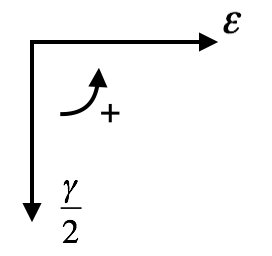
\includegraphics[scale=0.5]{annexes/rappels/TP3-1}
\end{wrapfigure}	
\ \\ Même principe que pour les tenseurs de contraintes. On commence par tracer les axes (où $\epsilon$ est l'axe des déformations longitudinales et $\frac{\gamma}{2}$ l'axe des déformations angulaires)\\\\

\begin{itemize}	
	\item On connaît cette fois $a_{ij} = 
	      \left(	
	      \begin{array}{cc}
	      	\epsilon _x             & \frac{1}{2}\gamma _{xy} \\ 
	      	\frac{1}{2}\gamma _{xy} & \epsilon _y             
	      \end{array}
	      \right) $
	      	
	\item On représente $x(\epsilon _x,\gamma _{xy})$ et $y(\epsilon _y ,\gamma _{xy})$ dont les composants sont en \textit{microstrenght}
\end{itemize}

\subsection*{Tenseurs des déformations évanouissantes}
\begin{equation}
	a_ {ij} = 
	\left(
	\begin{array}{ccc}
		\epsilon _x             & \frac{1}{2}\gamma _{xy} & \frac{1}{2}\gamma _{xz} \\ 
		\frac{1}{2}\gamma _{xy} & \epsilon _y             & \frac{1}{2}\gamma _{yz} \\ 
		\frac{1}{2}\gamma _{xz} & \frac{1}{2}\gamma _{yz} & \epsilon _z             
	\end{array} 
	\right)
	\qquad \qquad
	a_{ij} = \frac{1}{2}(a_{i,j} + a_{j,i})
\end{equation}

\subsection*{Formules utiles}
\begin{itemize}
	\item Tenseur des rotations
	      \begin{equation}
	      	\mu _{[i,j]} = \frac{1}{2}(\mu _{i,j} - \mu _{j,i})
	      \end{equation}
	      		
	\item Déformation axiale dans la direction $\vec{\nu}$
	      \begin{equation}
	      	\vec{\nu} = \nu _i \overline{1}_{x_i} \rightarrow \epsilon _{\nu} = a_{ij} \nu _j \nu _i
	      \end{equation}
	      		
	\item	Angle après déformation 
	      \begin{equation}
	      	\gamma _{\nu \mu} = 2 a_{\nu \mu} = 2 a_{ij} \nu _j \mu _i \rightarrow angle = \frac{\pi}{2} - \gamma _{\nu \mu} 
	      \end{equation}
	      \textbf{Remarque :} $\Delta L = L.\epsilon$		
	\item Loi de Hooke
	      \begin{equation}
	      	a_{ij} = \frac{1}{E}[(1+\nu)\tau _{ij} - \nu \delta _{ij}\tau _{kk}]
	      \end{equation}							
\end{itemize}

\subsection*{Remarque}
\begin{wrapfigure}[7]{l}{5cm}
	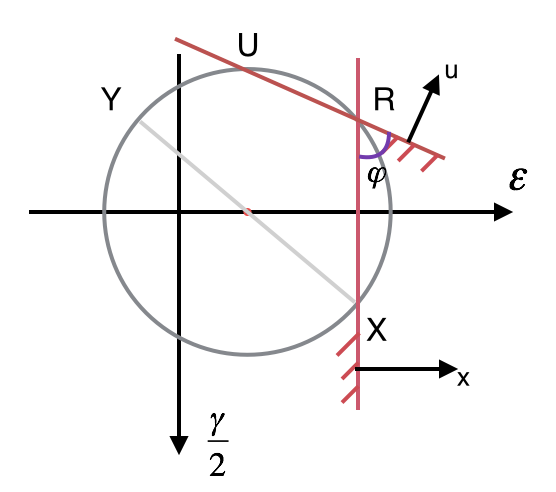
\includegraphics[scale=0.5]{annexes/rappels/TP3-2}
\end{wrapfigure}
\ \\ Durant ce tp on utilise le \textit{point de rayonnement} (intersection de la verticale passant par \textit{x} avec le cercle). Cela nous permet de mesurer directement l'angle $\varphi$ et non $2 \varphi$, mais aussi de représenter directement le plan physique sur le dessin (généralement on représente le vecteur physique du même côté que le point).\\


